\documentclass[11pt,a4paper]{extarticle}
\usepackage[utf8]{inputenc}
\usepackage[spanish]{babel}
\usepackage{amsmath}
\usepackage{amsfonts}
\usepackage{amssymb}
\usepackage{graphicx}
\usepackage[left=1.2cm,right=1.2cm,top=2cm,bottom=2cm]{geometry}
\date{\small{\today}}
\usepackage{fancyhdr}
\usepackage{afterpage}
\usepackage{titlesec}
\usepackage{float}
\usepackage{gensymb}
\usepackage{xfrac}
\usepackage{tabularx}
\usepackage{multicol}
\usepackage[font=small]{caption}
\usepackage{scrextend}
\usepackage[toc,page]{appendix}

\renewcommand\appendixpagename{Apéndices}
\renewcommand\appendixname{Apéndice}

\titleformat{\section}{\Large\bfseries}{}{0em}{}[]
\titleformat{\subsection}{\large\bfseries}{}{0em}{}[]
\titleformat{\subsubsection}{\bfseries}{}{0em}{}[]
\titleformat{\chapter}{\large\bfseries}{}{0em}{}[]


\setlength\parindent{0pt}


\begin{document}
\title{Amplificador Lock-In Digital}
	\LARGE{\textsc{Laboratorio II}}\\
	\Large{Amplificador Lock-In Digital}\\
\begin{large}
\small\textsc{Horst, Raúl Tomás}\\
\small\textsc{Roqueta, Matías Daniel}\\
\small{Centro Atómico Bariloche y Instituto Balseiro, Comisión Nacional de Energía Atómica}\\
\end{large}
\setcounter{page}{1}

\lhead{Laboratorio II}%Materia
\rhead{Medición de Impedancias con Amplificador Lock In}%Título 
\chead{}

\lfoot{R. Horst, M. Roqueta}
\cfoot{Instituto Balseiro} 
\rfoot{\thepage} 
\renewcommand{\headrulewidth}{0.4pt} 
\renewcommand{\footrulewidth}{0.4pt} 
\pagestyle{fancy}

\hrule
\begin{multicols}{2}
\normalsize
\section{Resumen}

\section{Introducción}

\begin{figure}[H]
	\centering
	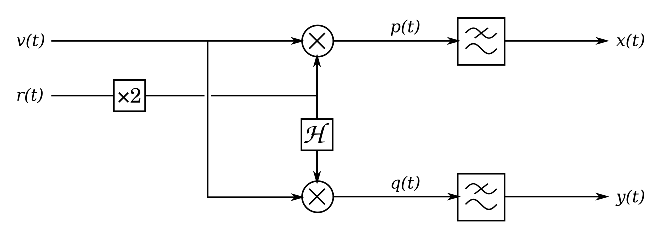
\includegraphics[width=\linewidth]{Images/lockin.eps}
	\caption{es un lockin}
	\label{fig:lockin}
\end{figure}


En la figura \ref{fig:lockin} hay un lockin

\section{Método Experimental}
En primer lugar se midió la frecuencia máxima de 
sampleo que permitía el dispositivo de medición.\\

Luego se ensambló el circuito de la F1. sobre 
un protoboard. Con ésto se evaluó el funcionamiento del
lock-in en un circuito de carácter puramente resistivo 
en donde se pudo obtener el valor de la resistencia 
de carga RL.\\ 

Se utilizaron dos generadores de señal RIGOL DG4102 
para poder generar la señal de referencia y el ruido.
Para sumar éstas dos señales se tuvo que "flotar"[1] la 
tierra de uno de los generadores dado que éstos no poseen 
tierra propia, sino que utilizan la de la red eléctrica.\\

Para la realización del lock-in se implementó un 
script en python como se puede ver en el apéndice.
En el código se importó la librería del dispositivo 
de medición, el 
conversor analógico dígital USB-1408FS de la línea 
MEASUREMENT COMPUTING para poder 
calibrarlo y realizar las mediciones.\\

Se implementaron 
las etapas de la figura \ref{fig:lockin}, en donde 
se optó por utilizar filtros FIR dada su versatilidad 
y sencillez.\\

El programa toma la señal v(t)
y la normaliza utilizando su máximo valor de amplitud,
 siendo ésta la tensión de referencia. Además se mide 
 la señal r(t) y se le aumenta la amplitud en un factor
 de 2 por el desarrollo que se necesita [Apéndice].
Se genera la señal p(t) mediante la multiplicación de 
las dos señales tomadas.
Luego se genera la señal q(t) desfasando 90◦
la señal 
mediante la transformada de Hilbert.
Por último se aplican filtros pasa bajos,
 obteniendo respectivamente las salidas x(t) e y(t),
  necesarias para obtener los
valores de amplitud y fase de la señal v(t).


\section{Resultados}

Falta analizar que puntos usar de las gráficas y reportar
el valor RL = ... +/- ..., CL = ... +/- ...
Se podría hacer un promedio de los valores, y el error hay 
que ver como pingo calcularlo/maquillarlo\\
Se determinó que la frecuencia máxima de muestreo es 
de aproximadamente 
500Hz, con una frecuencia máxima medible de 250Hz, 
según el teorema de muestreo de Nyquist[2].\\

Se midió el valor de RL en función 
de la relación señal a ruido en la entrada para tres 
filtros FIR de distinto orden.
Se puede apreciar que el filto óptimo es el de mayor 
orden, dado que se utilizan mayor cantidad de 
mediciones para generar las señales medidas.

\begin{figure}[H]
	\centering
	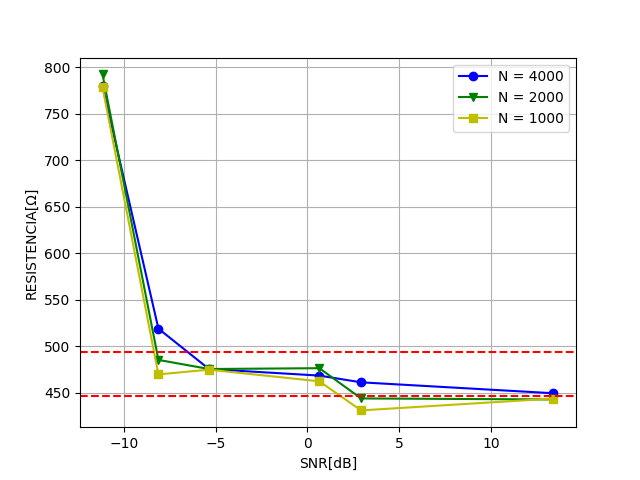
\includegraphics[width=\linewidth]{Images/RvsSNR(segunda).png}
	\caption{RvsSNR}
	\label{fig:RvsSNR}
\end{figure}

Para comprobar que el límite de funcionamiento 
del lock-in no está limitado por el orden del 
filtro elegido sino por la SNR a la entrada
se realizaron distintas mediciones 
sobre el valor RL(dada la simpleza del circuito) 
para un valor de SNR a la entrada de -22.5dB para 
distintos filtros como se explaya en la figura 
\ref{fig:RORDEN}. Se aprecia un valor mas acercado 
al tabulado cuando se aumenta el orden del filtro, sin 
embargo está lejos de entrar en la cota del error 
tabulado, y ésto afirma que el limitante en éste 
lock-in es el ruido a la entrada.\\

ESTARIA BUENO QUE EL ULTIMO PTO DE LA GRAFICA \ref{fig:RORDEN}
ESTE MAS ARRIBA PARA PODER HACER ESTA AFIRMACION 
VER SI CONVIENE PONER EN A TRABAJO FUTURO O MOVER EL PTO\\

Cabe aclarar que los valores de resistencia que estamos
 midiendo están dos ordenes de magnitud por de 
 bajo de la impedancias de entrada del dac, y al ser 
una conexión en paralelo predomina el valor de la resistencia 
que deseamos obtener.\\

\begin{figure}[H]
	\centering
	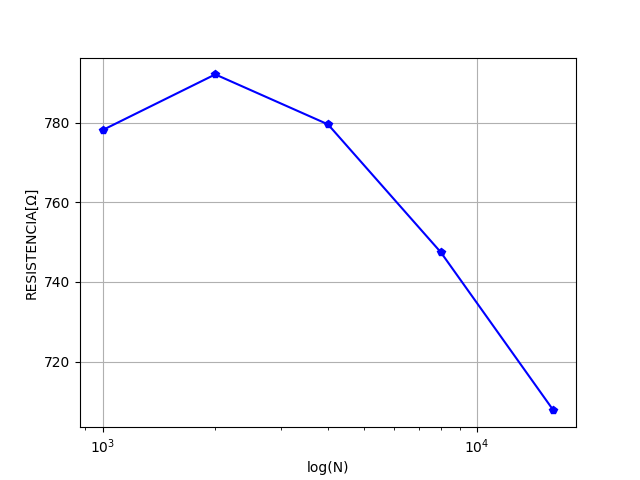
\includegraphics[width=\linewidth]{Images/RORDEN.png}
	\caption{RORDEN}
	\label{fig:RORDEN}
\end{figure}

Por último se armó el circutio de la figura 
\ref{fig:CvsSNR} .Con ésto 
se midió el valor de la capacidad CL para poder 
comprobar el funcionamiento del lock-in en 
impedancias complejas.\\ 

\begin{figure}[H]
	\centering
	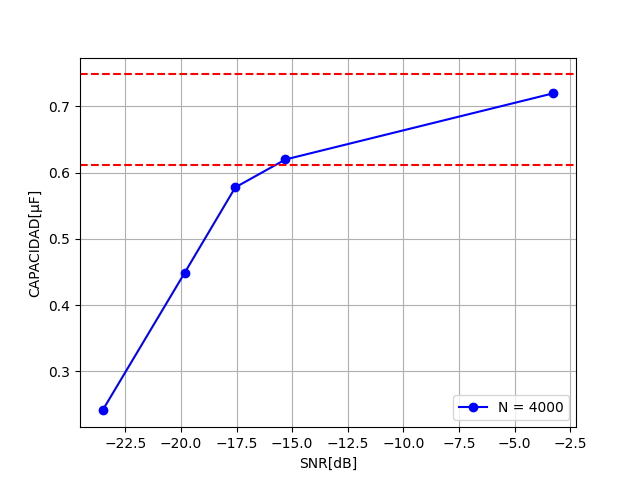
\includegraphics[width=\linewidth]{Images/CvsSNR(segunda).png}
	\caption{RvsSNR}
	\label{fig:CvsSNR}
\end{figure}


\section{Discusión}
-Orden del filtro\\
-Pq usamos FIR y no IIR\\
-Frecuencia de muestreo->usar otro dac\\
-Pq tuvimos que flotar\\
-Hacer más mediciones en el capacitor entre -5dB y -15db, 
porque en la resistencia llega hasta -12dB como mínimo.
Con respecto a ésto, ¿descartamos 4 puntos en el gráfica de 
la capacitancia?, nos queda sólo 1 :(

\section{Conclusiones}

Si bien los amplificadores lock-in comerciales resuelven 
mediciones con SNR de 1:1000(VER), se encuentra satisfactorio 
el rendimiento del lock-in digital desarrollado, con 
una implementación relativamente sencilla.\\

Se concluye que la mínima SNR de entrada para el 
correcto funcionamiento del lock-in implementado es de 
aproximadamente unos -6dB.(VER BIEN QUE VALOR DECIR, 
en dB o en 1:10 por ejemplo)

\section{Referencias}

\bibliography{Antenas}
\bibliographystyle{ieeetr}

\end{multicols}
\newpage
\begin{appendices}
\vspace{-1em}
\hrule
\vspace{1em}
\normalsize
\section{Apéndice 1 - si pinta meter un apéndice}
\end{appendices}

\end{document}
